\documentclass[12pt]{article}

\usepackage[T1]{fontenc}
\usepackage[polish]{babel}
\usepackage[utf8]{inputenc}
\usepackage{lmodern}
\selectlanguage{polish}

\usepackage{graphicx}
\usepackage{tabularx, booktabs}
\usepackage{fancyhdr} 
\usepackage{geometry}
\usepackage{hyperref}
\usepackage{listings}
\usepackage{float} 
\usepackage{subfigure}

\usepackage{a4wide}

\geometry{left=15mm,right=25mm,%
bindingoffset=10mm, top=20mm, bottom=20mm}
 


\renewcommand{\maketitle}{
\begin{titlepage}
\begin{table}[t]
\centering
\begin{tabular}[t]{lcr}
 
\includegraphics[width=70pt,height=70pt]{PW} & POLITECHNIKA WARSZAWSKA & 
\includegraphics[width=70pt,height=70pt]{MiNI}\\
& WYDZIAŁ MATEMATYKI & \\
& I NAUK INFORMACYJNYCH &
\end{tabular}
\end{table}
\vspace*{3cm}
  \begin{center}
    \LARGE
    \textbf {MSI2 - Raport}\\
   \vspace*{2 cm}
\begin{table}[!htp]
\begin{tabular}{p{4cm}p{9cm}}
\textit{Przedmiot:} &\textbf {Metody sztucznej inteligencji 2} \\
\\
\textit{Projekt:} &\textbf {Agent do grania w gry Atari przy użyciu uczenia wzmocnionego (reinforcement learning)} \\
\\
\textit{Autorzy:} &\textbf {Michał~Kołodziej \newline Nikodem~Wiśniewski} \\
\\
\end{tabular}
\end{table}

\vspace{5 cm}
  \center{\small Warszawa, dnia \today}
\end{center}
\end{titlepage}
}

\begin{document}
\maketitle

\tableofcontents

\newpage

\section{Opis projektu}
Zadaniem tego projektu jest stworzenie agenta komputerowego, grającego w gry z Atari 2600 \cite{atari}. Agent trenowany jest za pomocą uczenia przez wzmacnianie (reinforcement learning), poprzez samoczynne granie w wybrane gry. Agent, ze względu na długi czas trenowania, miał styczność tylko z jedną grą: Breakout. Ten sam model sieci powinien z powodzeniem posłużyć do nauki i gry w inne tytuły z konsoli Atari, bez potrzeby zmiany któregokolwiek z parametrów.

\section{Metodyka}

Do implementacji tego projektu użyty został język \textit{Python 3.6} w połączeniu z frameworkiem \textit{Keras} \cite{keras}, który wykorzystuje do obliczeń bibliotekę \textit{tensorflow} \cite{tensorflow}. \\
Do uczenia agenta użyte zostało środowisko OpenAI Gym \cite{gym} z rozszerzeniem o symulator gier Atari. Środowisko to udostępnia API do wyświetlania ekranu emulatora, wykonywania kolejnych akcji w emulatorze, resetowania stanu gry, pobierania informacji z emulatora, takich jak: zrzut ekranu emulatora, informacja o nagrodzie po wykonaniu akcji, informacja o zakończeniu się rozgrywki. Podczas uczenia agent ma przedstawione jako stan 4 ostatnie klatki z gry, na podstawie których wybiera akcje do wykonania w danym stanie. Dzięki temu ma on nie tylko podgląd obecnego zrzutu ekranu, ale również widzi dynamiczne zmiany zachodzące w grze. Z emulatora pobierane są zrzuty w rozmiarze $160\times210$ pikseli w przestrzeni barw RGB. W celu ograniczenia ilości przetwarzanych danych rozmiar każdej klatki jest skalowany i obcinany do $84\times84$ pikseli, a 3 kanały koloru są rzutowane na jeden kanał w 256 wymiarowej skali szarości.
\\\

\begin{figure}[H]%
\centering
\subfigure[Klatka z emulatora]{%
\label{fig:first}%
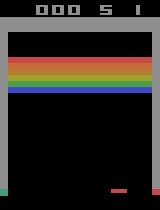
\includegraphics[scale=0.5]{1_raw.jpg}}%
\qquad
\subfigure[Klatka w skali szarości]{%
\label{fig:second}%

\includegraphics[scale=0.5]{2_gray.jpg}}%
\qquad
\subfigure[Klatka przeskalowana]{%
\label{fig:third}%

\includegraphics[scale=0.5]{3_resized.jpg}}%
\qquad
\subfigure[Klatka obcięta]{%
\label{fig:fourth}%

\includegraphics[scale=0.5]{4_cropped.jpg}}%
\caption{Kolejne kroki przetwarzania obrazu wejściowego}
\end{figure}


\subsection{Nagrody}

Na poączątku należy zdefiniować pojęcie nagrody w kontekście nauczania ze wzmocnieniem. Agent za każdą akcję dostaję nagrodę i dąży do maksymalizacji nagród w trakcie jednej gry. Aby uniezależnić agenta od konkretnych gier (każda gra ma swoją skalę punktacji), nagroda przedstawiana agentowi za każdy jego ruch jest wynikiem funkcji $sgn(reward)$. Końcowy wynik agenta możemy określić jako sumę nagród po wykonaniu n akcji:

$$R=r_1 + r_2 + r_3 + \dots + r_n$$

Na tej podstawie jesteśmy w stanie zdefiniować równanie sumy nagród uzyskanych w przyszłości zaczynając od momentu $t$:

$$R_t=r_t + r_{t+1}+ r_{t+2} + \dots + r_n$$

Niestety w środowisku Atari niektóre zachowania gier są losowe, przez co należy zaburzyć tą sumę zmniejszając nagrody proporcjonalnie do ich oddalenia w przyszłości, gdyż są one mniej pewne niż nagrody za najbliższe kroki agenta. Można wówczas skorzystać z równania na sumę nagród z \textit{rabatem}:

$$R_t=r_t + \gamma r_{t+1}+  \gamma^2 r_{t+2} + \dots + \gamma^{n-t}r_n$$

W sumie z \textit{rabatem} nagrody są pomniejszane o czynnik $\gamma$, który jest liczbą z przedziału $[0,1]$ , gdzie dla $\gamma =0$ strategia jest krótkoterminowa i pod uwagę brana jest tylko najbliższa nagroda, zaś wykorzustując $\gamma =1$ należałoby przyjąć, iż środowisko jest deterministyczne i kolejne akcje zawsze wywołują te same stany.

\subsection{Q-learning}

Do wyliczania kolejnych ruchów agenta użyty został \textbf{Q-learning}. Zdefiniujmy więc funkcję \textit{Q(s,a)}, gdzie \textit{s} to stan, zaś \textit{a} to akcja możliwa do wykonania w danym stanie. Funkcja ta reprezentuje możliwie największy wynik pod koniec gry, w przypadku podjęcia akcji \textbf{a} w stanie \textbf{s}. Określona jest ona rekurencyjnym równaniem Bellmana:

$$Q(s,a) =  r + \gamma max_{a'}Q(s',a')$$

gdzie $r$ to nagroda po wykonaniu akcji $a$ w stanie $s$, $\gamma$ to współczynnik rabatu, $s'$ to stan, w którym znajdziemy się po wykonaniu akcji $a$, zaś $a'$ to kolejna optymalna akcja.

\subsection{Deep Q-network}

W związku z tym, że każda z 4 ostatnich klatek gry ma rozdzielczość $84\times 84$, a każdy piksel może mieć 256 możliwych wartości w skali szarości, mamy wówczas $256^{84\times84\times4}$ stanów gry. Jest to tak ogromna liczba, że nie jesteśmy w stanie stworzyć tablicy do zapamiętania funkcji Q.
W celu skutecznego wyliczania i aproksymowania wartość funkcji $Q(s,a)$ użyta została sieć neuronowa. Naturalną implementacją takiej sieci byłoby przyjęcie na wejściu stanu gry oraz wybranej akcji, wówczas w odpowiedzi wyliczana by była jakość tej akcji w danym stanie. Bardziej optymalnym podejściem jest stworzenie sieci, która na wejściu przyjmuje stan gry (4 klatki z gry), a na wyjściu zwraca wartość funkcji Q dla każdej możliwej akcji w danym środowisku. Dzięki takiej architekturze tylko jedno wyliczenie wskazuje optymalną akcję. W przeciwnym wypadku ilość obliczeń uzależniona jest liniowo od ilości akcji. W Atari 2600 mamy 18 możliwych akcji do wykonania (chociaż nie wszystkie są używane we wszystkich grach).
\\
Dla każdego przejścia $<s, a, r, s'>$ aktualizujemy naszą sieć następującym algorytmem:
\begin{enumerate}
\item Wykonujemy feedforward dla poprzedniego stanu $s$, aby uzyskać przewidywaną Q-wartości dla akcji $a$. Oznaczmy więc wyliczoną w ten sposób wartość $Q'(s,a)$.
\item Wykonujemy feedforward dla obecnego stanu $s'$ i wybieramy wartość dla najlepszej akcji $max_{a'}Q(s',a')$.
\item Wyliczamy poprawną wartość funkcji $Q$ dla akcji $a$ korzystając ze wzoru: $$Q(s, a) = r + \gamma max_{a'}Q(s',a')$$ Dla pozostałych akcji zostawiamy wartość funkcji $Q$ uzyskaną z naszej sieci.
\item Liczymy funkcję straty (loss function) wzorem: $$L=\frac{1}{2}[Q(s,a)-Q'(s,a)]^2=\frac{1}{2}[r+\gamma max_{a'}Q(s',a')-Q'(s,a)]^2$$ Uwaga: funkcja straty dla akcji innych niż $a$ przez powyższe założenie wynosi 0. 
\item Aktualizujemy wagi w sieci używając wstecznej propagacji (backpropagation).
\end{enumerate}

\subsection{Dodatkowe założenia i metody}

\subsubsection{Experience replay}

Podczas grania kolejne stany są często bardzo podobne i mało się różnią. Powoduje to, że sieć zbiega się rozwiązaniami dla konkretnej części rozgrywki i wpada w maksimum lokalne (np. dla gry Breakout sieć zaczyna faworyzować ruchy paletką w jednym z dwóch kierunków). Aby temu zapobiec, w trakcie gry ostatnie milion doświadczeń w postaci krotek $<s, a, r, s'>$ zapisywanych jest w pamięci zwanej dalej \textit{pamięcią doświadczeń}. Przy trenowaniu sieci nie jest używane ostatnie doświadczenie, ale losowa porcja próbek doświadczeń z pamięci. W ten sposób łamane jest podobieństwo kolejnych stanów, przypominając sieci wszelkie pamiętane elementy rozgrywki, nie tylko sekwencyjne.
\\\

W przeciwieństwie do oryginalnej pracy zespołu Deepmind \cite{deepmind_2}, w tej pracy sieć nie jest uczona na podstawie $n$ losowych doświadczeń, ale na podstawie sumy najświeższego doświadczenia z liczbą $n-1$ losowych krotek. Zabieg ten ma na celu przyspieszenie i ulepszenie nauki w dalszych etapach rozgrywki. W większości gier liczba możliwych stanów rośnie wraz z rozwojem rozgrywki (tudzież zdobyciem większej ilości punktów) wykładniczo. Wówczas dalsze stany gry są dużo rzadziej osiągane, co za tym idzie - mają dużo mniejsze prawdopodobieństwo wylosowania przy nauczaniu sieci. Może to w konsekwencji powodować zbyt mały wpływ zaawansowanych stanów gry na naukę sieci, czego wynikiem będzie spowalnianie szybkości uczenia wraz z upływem czasu.
\\
Rozumowanie to jest czysto teoretyczne i nie ma formalnego dowodu.

\subsubsection{Exploration-exploitation dilemma}

Podczas inicjalizacji sieć wypełniania jest losowymi liczbami, więc początkowo wybierane akcje również będą losowe. Jest to czysta eksploracja. W przypadku, gdy nasza sieć zbiega się do niektórych rozwiązań algorytm zatrzymując się w maksimum lokalnym nie będzie przeszukiwał nowych ścieżek i zachowań zadowalając się uzyskanym wynikiem. Aby temu zapobiec, wykorzystana została metoda z $\varepsilon\ greedy\ exploration$ - każdy ruch wybierany jest z prawdopodobieństwem $\varepsilon$ na wykokanie losowej akcji.

\subsubsection{Network freezing}

W związku z tym, iż funkcja straty wykorzystuje sieć neuronową, dla której jest liczona, co jest pewnego rodzaju rekurencją - do poprawy sieci neuronowej wykorzysujemy wyniki z niej samej. Taka zależność może powodować wolniejsze zbieganie się wyników do oczekiwanych. Przypomnijmy wzór: 

$$L=\frac{1}{2}[Q(s,a)-Q'(s,a)]^2=\frac{1}{2}[r+\gamma max_{a'}Q(s',a')-Q'(s,a)]^2$$

Aby ustabilizować zbieganie się modelu, co określoną liczbę iteracji zapisywany jest jego stan. Jest to tak zwana metoda mrożenia sieci. Za pomocą tej pomocniczej zamrożonej sieci przewidywane są wartości rekurencyjne z funkcji straty. Takie działanie powoduje znaczną poprawę szybkości uczenia się modelu i jego stabilności.

\section{Architektura sieci \cite{deepmind_2}}

Sieć neuronowa wykorzystana w tej pracy jest tradycyjną siecią konwolucyjną z trzema warstwami konwolucyjnymi i jedną warstwą w pełni połączoną. Wejściowy stan postaci $84\times84\times4$ trafia do pierwszej warstwy konwolucyjnej złożonej z 32 filtrów rozmiaru $8\times8$ o kroku (\textit{stride}) 4 na wyjściu, przechodząc przez funkcję ReLU. Druga warstwa konwolucyjną składa się z 64 filtrów $4\times4$ o kroku 2, po której wyniki są przepuszczane przez funkcję ReLU. Trzecia warstwa konwolucyjna składa się z 64 filtrów $3\times3$ o kroku 1, po której również jest funkcja ReLU. Ostatnią warstwą ukrytą jest w pełni połączona warstwa z 512 neuronami. Wyjściowa warstwa jest warstwą w pełni połączoną z wyjściem dla każdej możliwej akcji.

W celu normalizacji wyników różniących się w każdej z gier, nagrody zostały zmienione na 1 dla nagród pozytywnych, -1 dla nagród negatywnych oraz 0 w pozostałych wypadkach.

\begin{center}

\begin{table}[H]
  \centering%
  \caption{Lista parametrów}
\begin{tabular}{|p{3cm}|p{3cm}|p{10cm}|}
\hline
\textbf{Parametr} & \textbf{Wartość} & \textbf{Opis} \\
\hline

batch size &
32 & 
Rozmiar porcji, na podstawie której sieć jest ulepszana. \\
\hline

początkowa eksploracja &
1 &
Początkowe $\varepsilon$ w eksploracji $\varepsilon$-greedy. \\
\hline

końcowa eksploracja &
0.1 &
Ostateczne $\varepsilon$ w eksploracji $\varepsilon$-greedy. \\
\hline

ostatnia klatka eksploracji &
1 000 000 &
Liczba klatek, w trakcie których wartość $\varepsilon$ jest zmniejszana liniowo z wartości początkowej do końcowej.\\
\hline

rabat &
0.99 &
Wartość $\gamma$ rabatu w algotytmie Q-learning.\\
\hline

liczba omijanych klatek &
4 &
Każda wybrana akcja wykonywana jest na określonej liczbie kolejnych klatek w celu uspójnienia ruchów agenta. \\
\hline

rozmiar pamięci doświadczeń &
1 000 000 &
Liczba doświadczeń trzymanych w buforze pamięci.
\\
\hline

mrożenie sieci &
10 000 &
Liczba iteracji, po których mrożona jest sieć i zapisywana jej kopia do wyliczeń celu.  \\
\hline

metoda gradientu &
RMSProp &
Algorytm wykorzystywany przy aktualizacji sieci neuronowej.  \\
\hline

learning rate &
0.00025 &
Współczynnik nauczania stosowany przez metodę gradientu.  \\
\hline

rho &
0.95 &
Współczynnik rho stosowany przez metodę gradientu.  \\
\hline

epsilon &
0.01&
Współczynnik epsilon stosowany przez metodę gradientu.  \\
\hline

\end{tabular}
\end{table}
\end{center}

\begin{figure}[H]
\centering 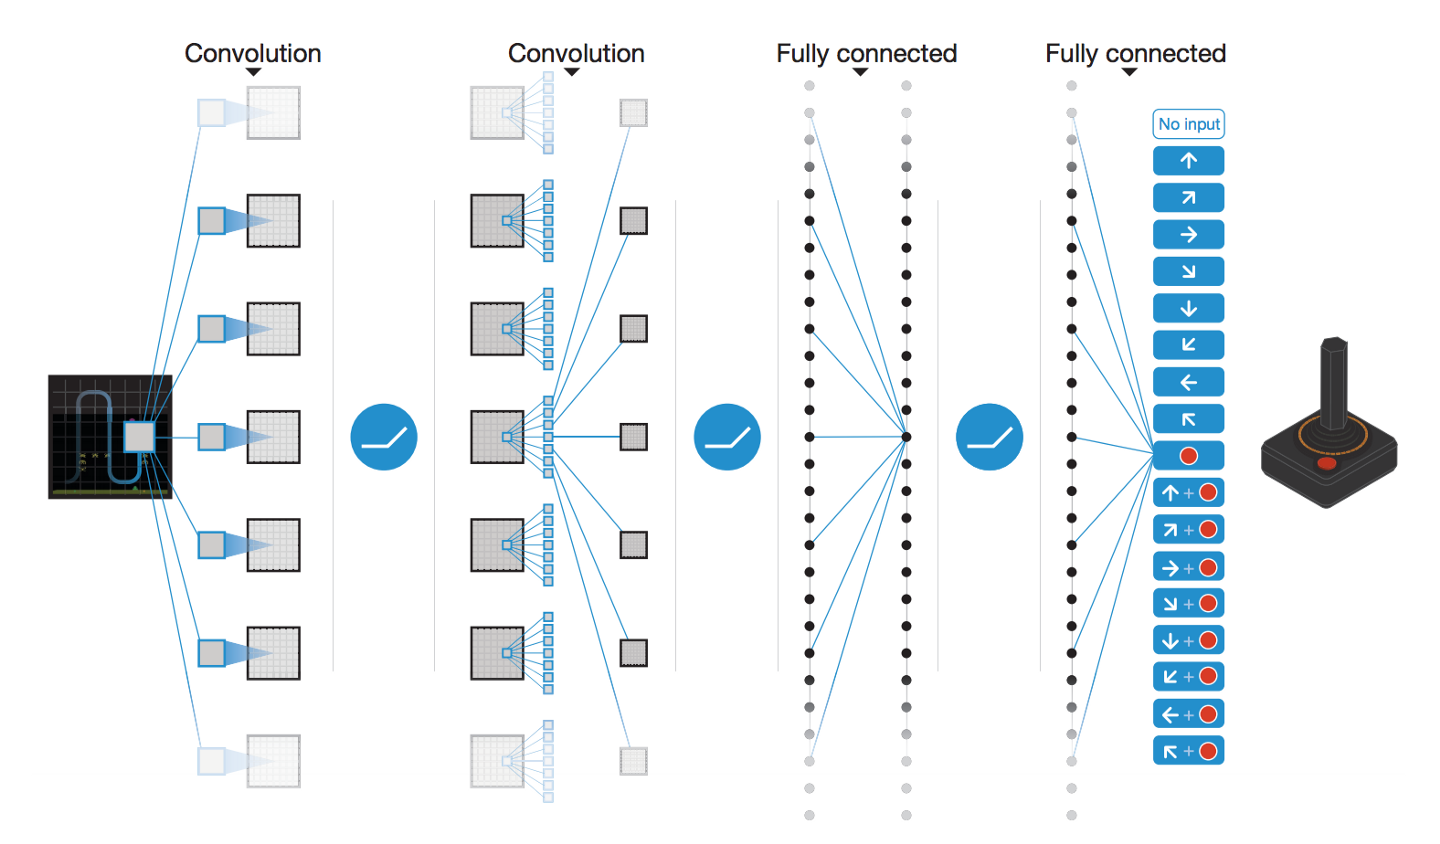
\includegraphics[scale=0.3]{network.png}
\caption{Schemat sieci neuronowej. \cite{deepmind_2}}
\label{simple1}
\end{figure}

\subsection{Algorytm trenowania}

\begin{lstlisting}
 initialize replay memory D
 initialize the neural network with random data
 get the current state 's'
 while game not over
 	if random > epsilon 
 		'a' = random action
 	otherwise
 		'a' = argmax_{a'}Q(s,a')

	perform action 'a'
	get reward 'r' and state 's`'
	store experience <s,a,r,s'> in memory D
	
	sample 32 random experiences <ss, aa, rr, ss'> from memory D
	for each experience from the sample batch
		if ss' is the final state 
			tt=rr
		otherwise
			tt=rr+gamma*argmax_{aa'}Q(ss', aa')
	
	optimize the neural network using loss function tt-Q(ss,aa))^2
	
	s=s'
\end{lstlisting}

\newpage

\section{Wyzwania}
\subsection{Pamięć doświadczeń}
Podczas nauki z pamięci doświadczeń pobierana jest porcja losowych doświadczeń. Każde doświadczenie złożone jest ze stanu gry, akcji, nagrody oraz następnego stanu. Każdy stan gry składa się z 4 klatek gry w skali szarości, rozmiaru $84\times84$ pikseli. Podczas implementacji pamięci doświadczeń należy mieć na uwadze, że pamiętanych ma być n ostatnich doświadczeń. Do takiego celu warto użyć $ring buffer$. Cała pamięć doświadczeń jest zapamiętywana w pamięci RAM, co w połączeniu z jej dużym rozmiarem (1 000 000) powoduje konieczność optymalizacji. Ze względu na mały rozmiar nagrody oraz akcji pamiętanych w każdym z doświadczeń, ich wpływ na rozmiar całej pamięci jest pomijalny.

Największym narzutem w pamięci doświadczeń są zrzuty ekranu z gry. W każdym stanie są aż 4 takie zrzuty. Należy pamiętać, że do zapamiętania każdego z pikseli wystarczy użycie 8 bitowej komórki pamięci, która daje możliwość zapisu 255 wartości. Implementując program w Pythonie z użyciem biblioteki NumPy można skorzystać z typu $uint8$. Ten sam typ warto wykorzystać do zapamiętania nagrody oraz akcji każdego doświadczenia. Wykonanie takich kroków nie daje jeszcze satysfakcjonujących wyników, ponieważ pamięć z milionem doświadczeń w takiej konfiguracji przekracza 110GB zajętej pamięci.
\\\

 \textbf{Uwaga:} domyślnym typem w tablicy NumPy jest 64 bitowy $float64$, przez co bez rzutowania explicité otrzymuje się 8 razy większą pamięć doświadczeń niż optymalnie. 
\\\

Do wykonania kolejnych optymalizacji należy przyjrzeć się dokładniej stanom gry. Stan gry składa się z 4 kolejnych klatek gry $s=\{A, B, C, D\}$, następujący po nim stan s’ zawiera jeden nowy zrzut ekranu $s’=\{B, C, D, E\}$. Widać więc, że do zapamiętania każdego stanu (poza pierwszym)  potrzeba odłożyć w pamięci tylko jeden nowy zrzut ekranu, dla reszty korzystając z referencji do pamięci już zaalokowanej. Dzięki temu, że nowy stan z doświadczenia $i$ jest starym stanem z doświadczenia $i+1$, zapamiętanie nowego doświadczenia wymaga zaalokowania pamięci na tylko jeden zrzut ekranu. Wówczas jedno doświadczenie to koszt pamięciowy jednego zrzutu ekranu $84\times84$ zamiast ośmiu obiektów tego typu. Dzięki temu uzyskać można 8-krotną optymalizację, a całość w połączeniu z poprzednimi poprawkami pozwala na zmieszczenie się wszystkich doświadczeń w około 10GB pamięci RAM.

\subsection{Moc obliczeniowa}
Dużym wyzwaniem dla realizacji tego projektu jest moc obliczeniowa. Do wytrenowania tak rozległej sieci na każdą z wybranych gier zespół Deepmind \cite{deepmind_2} poświęcał 50 milionów iteracji nauki, co sami wycenili na 38 dni nieprzerwanej gry agenta. Z tego względu eksperyment ten jest nie do powtórzenia w domowych warunkach bez stacji roboczej ze specjalistyczną kartą graficzną i pamięcią RAM o rozmiarze co najmniej 16GB. Warto zaznaczyć, że ze względu na specyficzne biblioteki \cite{gym} środowisko działa poprawnie tylko na systemach z rodziny GNU~/~Linux np. Ubuntu \cite{ubuntu}.  Alternatywą do nauczania agenta na domowych komputerach są ogólnodostępne chmury obliczeniowe. Istnieje kilka darmowych rozwiązań tego typu z ograniczoną ilością mocy obliczeniowej. Ze względu na duży narzut pamięci (10GB), jedyną pasującą spośród dostępnych opcji okazało się środowisko Google Colaboratory \cite{colab}. 
\\\

Środowisko to udostępnia moc obliczeniową karty graficznej NVIDIA Tesla K20 z dostępną pamięcią około 11GB. Program uruchomiony w tym środowisku wykonuje 50 000 iteracji nauki w około 40 minut, czyli milion iteracji nauki w około 13 godzin. Całość treningu dla jednej gry trwałaby ponad 27 dni. Niestety ze względu na to, że jest to rozwiązanie darmowe, ma ono swoje ograniczenia. Środowisko uruchamiane jest w przeglądarce internetowej z pomocą specjalnych skryptów o rozszerzeniu \textit{ipynb} (skrypty Jupyter notebook \cite{jupiter}). Aby uruchomić skrypt należy otworzyć plik w przeglądarce z poziomu Google Drive \cite{drive}, pozostawiając otwarte okno przeglądarki na cały czas pracy skryptu. Wykonujący się proces programu może w dowolnym momencie zostać zabity. Jest to zależne od liczby innych użytkowników współdzielących zasoby tego środowiska. Ograniczony jest również maksymalny czas obliczeń, po którym maszyna wirtualna, do której jest się podłączonym, zostaje wyłączona. W praktyce można zauważyć, że jest to około 15 godzin. 
\\\

Ze względu na taką charakterystykę środowiska obliczeniowego, uczenie sieci w jednej ciągłej sesji okazało się niemożliwe. Aby temu zaradzić, skrypt uczący co określoną liczbę iteracji zapisuje kopię modelu sieci do pliku. Dzięki temu po przerwanych obliczeniach można je wznowić od wyznaczonego momentu. Niestety podczas wznawiania obliczeń z zapisanego modelu tracona jest cała pamięć doświadczeń, która była zapisana w pamięci RAM. Może to mieć decydujący wpływ na szybkość i jakość nauczania agenta.


\section{Wyniki}
Ze względu na ograniczenia czasowe, sieć była uczona tylko na jednej grze - Atari Breakout \cite{breakout}. W grze tej dostępne są 4 akcje: bezruch, poruszenie paletką w lewo, poruszenie paletką w prawo oraz rzucenie piłeczki.




\begin{figure}[H]%
\centering
\subfigure{%
\label{atari:first}%
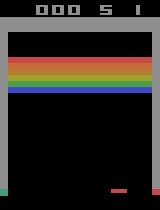
\includegraphics[scale=0.85]{1_raw.jpg}}%
\qquad
\subfigure{%
\label{atari:second}%
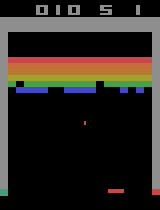
\includegraphics[scale=0.85]{during_game.png}}%
\qquad
\subfigure{%
\label{atari:third}%
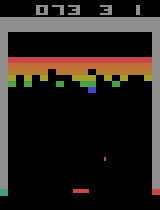
\includegraphics[scale=0.85]{during_game2.png}}%

\caption{Klatki z gry Atari Breakout granej przez model uczony przez 8 milionów iteracji}
\label{atari1}
\end{figure}



Gra polega na takim odbijaniu poruszającej się piłeczki sterowaną paletką, aby zbijać kolorowe klocki umieszczone w rzędach w górnej części ekranu gry (Rysunek \ref{atari1}).
\\
W celu oceny szybkości i jakości nauki, przeprowadzone zostały testy dla zapisanych w różnych etapach uczenia modeli. Każdy model gra określoną liczbę gier używając $\epsilon=0.05$. Wynikiem modelu jest uśredniony znormalizowany wynik z każdej z gier. 

\begin{center}
\begin{table}[H]
  \centering%
  \caption{Średnie wyniki zapisanych modeli w różnych etapach uczenia.}
\begin{tabular}{|c|c|}
\hline
\textbf{Liczba iteracji (tysiące)} & \textbf{Średni znormalizowany wynik}\\
\hline
0 &  4.95 \\
\hline
200  &  4.5 \\
\hline
600  &  5.0 \\
\hline
800  &  3.1 \\
\hline
1000  &  2.9 \\
\hline
1200  &  7.8 \\
\hline
1400  &  8.5 \\
\hline
1550  &  8.45 \\
\hline
1800  &  11.85 \\
\hline
2000  &  11.1 \\
\hline
2200  &  11.9 \\
\hline
2400  &  14.45 \\
\hline
2500  &  15.55 \\
\hline
2700  &  17.9 \\
\hline
3000  &  20.6 \\
\hline
3200  &  21.6 \\
\hline
3500  &  23.65 \\
\hline
3800  &  30.7 \\
\hline
4150  &  31.55 \\
\hline
4400  &  27.05 \\
\hline
4600  &  34.35 \\
\hline
4800  &  32.65 \\
\hline
5000  &  38.5 \\
\hline
5250  &  38.4 \\
\hline
5400  &  31.05 \\
\hline
5600  &  36.65 \\
\hline
5800  &  39.8 \\
\hline
6000  &  38.85 \\
\hline
6200  &  40.25 \\
\hline
6400  &  40.05 \\
\hline
6800  &  40.35 \\
\hline
7000  &  36.85 \\
\hline
7200  &  37.7 \\
\hline
7400  &  38.85 \\
\hline
7600  &  37.35 \\
\hline
7750  &  36.95 \\
\hline
8000  &  40.3 \\
\hline
\end{tabular}
\end{table}
\end{center}

\begin{figure}[H]
\centering 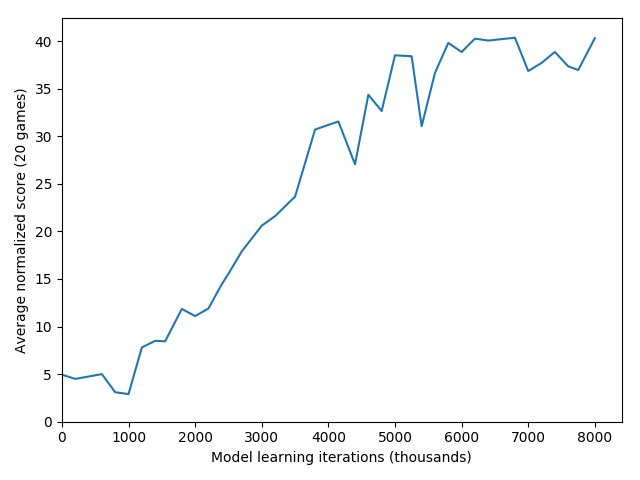
\includegraphics[scale=0.7]{20games.png}
\caption{Uśredniony znormalizowany wynik z 20 gier Breakout w stosunku do liczby iteracji nauki (w tysiącach).}
\label{results}
\end{figure}


 Jak widać, na Rysunku \ref{results} dla modelu grającego losowo, wynik jest niezerowy, co jest istotnym faktem do zanotowania. Na początku nauczania grający agent nie polepszał znacząco swoich wyników, a jego wynik nie różnił się od agenta grającego losowo. Skok średniej liczby punktów widoczny jest dopiero po ponad milionie iteracji nauki (około 13 godzin). Przez kolejne 3 miliony cykli agent uczył się z mniej więcej stałym tempem. Po tym czasie widoczne są już załamania i częściowe, chwilowe regresje w nauce. Po 5 milionach iteracji widoczne jest również znaczne spowolnienie trenowania i ustabilizowanie się wyniku. Jest to niepożądane i niespodziewane zachowanie, które może być spowodowane przerywanymi sesjami nauki z resetowanym stanem pamięci doświadczeń.

\section{Instrukcja obsługi}

Do uruchamiania programu potrzebny jest system operacyjny z zainstalowanym środowiskiem uruchomieniowym Python 3.6 oraz wymienionymi niżej modułami. Moduł \textit{gym[atari]} nie ma wsparcia dla systemu Windows, dlatego zalecane jest uruchamianie projektu na systemie Ubuntu. 
\\

Program uruchamiany jest poprzez wykonanie skryptu \textbf{game.py}.

\subsection{Moduły}
Lista wymaganych modułów:
\begin{itemize}
\item \textit{tensorflow} biblioteka do wykonywania obliczeń numerycznych;
\item \textit{keras} wysokopoziomowe API do tworzenia modeli sieci neuronowych;
\item \textit{gym} środowisko uruchomieniowe agenta;
\item \textit{gym[atari]} środowisko uruchomieniowe agenta;
\item \textit{h5py} biblioteka do zapisu i odczytu modeli sieci neuronowych z plików;
\item \textit{numpy} biblioteka do wykonywania operacji matematycznych;
\item \textit{skimage} biblioteka do manipulacji obrazami;
\item \textit{matplotlib} biblioteka do generowania wykresów.
\end{itemize}

\subsection{Pliki}
Pliki skryptowe używane w projekcie:
\begin{itemize}
\item \textit{game.py} główny plik uruchomieniowy służący do uczenia sieci;
\item \textit{atari\_model.py} skrypt z definicją sieci neuronowej oraz API do korzystania z niej;
\item \textit{env\_wrapper.py} skrypt z klasą opakowywującą dla środowiska uruchomieniowego agenta z dodatkowymi funkcjonalnościami;
\item \textit{helpers.py} zbiór funkcji pomocniczych;
\item \textit{ring\_buf.py} skrypt z klasą pamięci doświadczeń;
\item \textit{game\_benchmark.py} skrypt do oceny nauczonych modeli.
\end{itemize}

\subsection{Parametry}
Na początku pliku \textit{game.py} zadeklarowane są parametry służące do strojenia programu:
\begin{itemize}
\item \textit{GAME\_ENV\_NAME} nazwa środowiska gry atari (\href{https://gym.openai.com/envs/#atari}{lista dostępnych gier});
\item \textit{LEARN} flaga decydująca, czy sieć ma być uczona;
\item \textit{RENDER} flaga decydująca o wyświetlaniu emulatora Atari podczas grania;
\item \textit{SAVE\_MODEL\_PATH} ścieżka do miejsca cyklicznego zapisywania stanu sieci;
\item \textit{STARTING\_MODEL} ścieżka do zapisanego modelu, od którego mają rozpocząć się obliczenia lub \textit{None};
\item \textit{BATCH\_SIZE} rozmiar porcji doświadczeń używanych podczas jednej iteracji nauki;
\item \textit{MEMORY\_SIZE} rozmiar pamięci doświadczeń;
\item \textit{FREEZE\_ITERATIONS} liczba iteracji, co które kopia sieci jest zapisywana i podmieniana z siecią zamrożoną;
\item \textit{REPLAY\_START\_SIZE} liczba początkowych iteracji, podczas których agent się nie uczy (trwa zapełnianie pamięci doświadczeń);
\item \textit{LAST\_EPSILON\_DECREASE\_ITERATION} liczba iteracji liniowego zmniejszania wartości $\epsilon$;
\item \textit{START\_EPSILON} początkowe $\epsilon$;
\item \textit{END\_EPSILON} końcowe $\epsilon$;
\item \textit{REPORT\_ITERATIONS} liczba iteracji, co które na konsoli wyświetlają się informacje dotyczące przebiegu uczenia;
\item \textit{SAVE\_MODEL\_ITERATIONS} liczba iteracji, co które aktualny model jest zapisywany do pliku.
\end{itemize}

\subsection{Instrukcja do Google Colaboratory \cite{colab}}

W celu skorzystania z silnika obliczeniowego Google Colaboratory, należy umieścić w swoim Google Drive wszystkie pliki skryptowe oraz plik \textbf{atari.ipynb}. W tym celu w głównym katalogu Google Drive należy utworzyć oddzielny folder o nazwie \textbf{app}. Pozwoli to zachować porządek, ponieważ skrypt automatycznie generuje pliki nauczonych modeli. 
\\

Skrypt \textbf{atari.ipynb} podzielony jest na dwie części. Oba komponenty całkowicie kompletują środowisko uruchomieniowe instalując potrzebne zależności oraz podpinają Google Drive w maszynie wirtualnej pod ścieżką \textbf{./drive}. Aby skrypty i modele zostały odnalezione należy więc skonfigurować ścieżki do plików w skryptach, tak aby zaczynały się od~\textbf{./drive/app}.
\\

Pierwsza część skryptu odpowiada za uruchomienie skryptu \textit{game.py} służącego do trenowania modelu. Druga zaś jest odpowiedzialna za uruchamianie skryptu \textit{game\_benchmark.py} oceniającego zapisane modele.

\newpage

\begin{thebibliography}{9}

\bibitem{atari}
  Atari 2600 \url{https://en.wikipedia.org/wiki/Atari_2600}

\bibitem{keras}
Keras \url{https://keras.io/}

\bibitem{tensorflow}
Tensorflow \url{https://www.tensorflow.org/}

\bibitem{gym}
  OpenAI Gym \url{https://gym.openai.com/}

\bibitem{colab}
  Google Colaboratory \url{https://colab.research.google.com}

\bibitem{breakout}
  Atari Breakout \url{https://en.wikipedia.org/wiki/Breakout_(video_game)}

\bibitem{drive}
Google Drive \url{https://drive.google.com/drive/}

\bibitem{jupiter}
Jupiter notebook \url{http://jupyter.org/}

\bibitem{ubuntu}
Ubuntu \url{https://www.ubuntu.com/}

\bibitem{deepmind_1}
  Volodymyr Mnih et al. 
\textit{Playing Atari with Deep Reinforcement Learning.} Deepmind, 2013
   \url{https://deepmind.com/research/publications/playing-atari-deep-reinforcement-learning/}

\bibitem{deepmind_2}
  Volodymyr Mnih et al. 
\textit{Human-level control through deep reinforcement learning.} Deepmind, 2015
   \url{https://deepmind.com/research/publications/human-level-control-through-deep-reinforcement-learning/}


\end{thebibliography}


\end{document}